\def\PicPath{/Users/ken/Documents/shuron/chapter1/1_1}

\begin{comment}
ガンマ線ってこういうの MeVガンマ線はこういうエネルギーを持ったガンマ線
MeVガンマ線は例えば、こういうものから出ている、見えてくる
MeVガンマ線の特徴…大気に吸収されやすい、バックグラウンドが多い、観測装置を作るのが難しい
その結果他の領域に比べて遅れている
\end{comment}

\section{MeVガンマ線領域}
\subsection{多波長と比べた時のMeVガンマ線の特徴}
ガンマ線は数十keV以上のエネルギーを持つ電磁波を指すが、その範囲は非常に広く数TeVにまで及ぶ。その幅広い範囲のどの領域で観測するかによって見えてくる宇宙の現象は異なってくる。
例えば、超新星爆発時にばらまかれる放射性同位体からの核ガンマ線が丁度数MeVの領域であるため、MeVガンマ線を観測することによって元素合成の様子が直接観測できると期待されている。他にも多くの物理現象の詳しい描像を得られると期待されており、非常に興味深い領域となっている。

しかし、MeVガンマ線観測には様々な困難が存在する。
天体からのMeVガンマ線は地球大気によって地表に届くまでにほとんど吸収されてしまうため(図\ref{fig:atm_absp})、大気圏内で観測を行うには高度40km以上で観測可能な大気球、もしくは大気が存在しない宇宙空間での観測を実現する衛星を用いる他はない。
加えてX線と比較するとエネルギーが高い分光子数が少なく、宇宙空間における透過力も強いので、宇宙全体に広がってしまったガンマ線が存在しバックグラウンド源になってしまっている。さらに、この様な注目天体以外からのガンマ線が検出器本体と相互作用を起こしてバックグラウンドをより多くしてしまう。

こうした背景から様々な物理現象の解明に繋がると期待されていながらも、MeVガンマ線の観測は他の領域に比べると未開拓な部分が多い(図\ref{fig:science_sensitivity})。従ってMeVガンマ線領域はより感度の高い検出器・検出手法が求められている領域である。

\begin{figure}
\centering
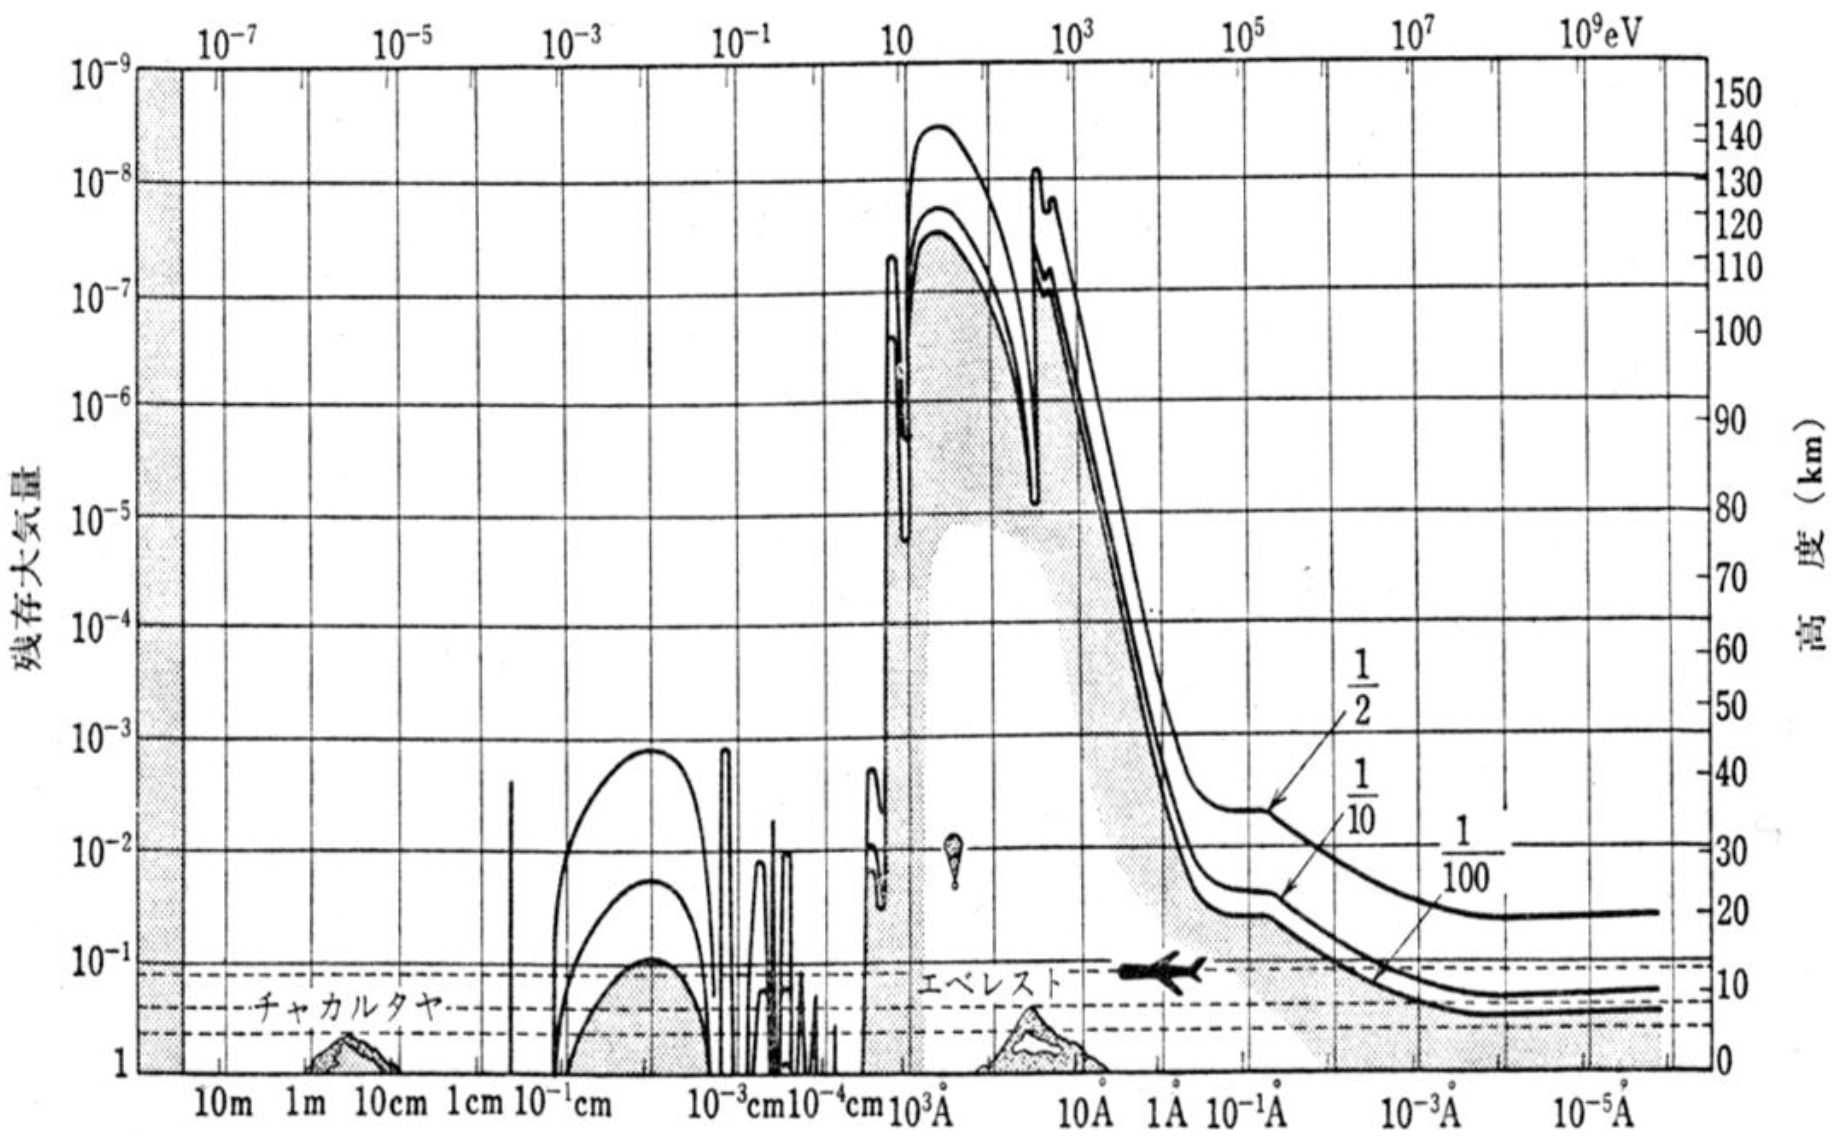
\includegraphics[width=15cm]{\PicPath/atmosphere_absorption.png}
\caption{大気による様々な波長の電磁波の吸収(出典??)\cite{oda_and_matsuoka}}
\label{fig:atm_absp}
\end{figure}

\begin{figure}
\centering
\includegraphics[width=15cm]{\PicPath/science_sensitivity.png}
\caption{X線・ガンマ線領域における現在までの観測及び到達感度(最新?)。破線はこれから観測が予定されているもので(最新?)、赤色の破線は京都大学の目標値である}
\label{fig:science_sensitivity}
\end{figure}

\clearpage